% journal_ui_ana/indonesia/src/40_hasil_pembahasan.tex
\section{Hasil dan Pembahasan}
\label{sec:hasil_jurnal_ui_ana}

Bagian ini menyajikan hasil analisis keamanan dan pengukuran performa, diikuti dengan diskusi mengenai temuan tersebut.

\subsection{Hasil Analisis Keamanan}
Efektivitas virtualisasi VxLang dievaluasi melalui upaya analisis statis dan dinamis untuk memahami dan mem-\textit{bypass} logika autentikasi pada aplikasi studi kasus.

\subsubsection{Analisis Statis (Ghidra)}
Analisis statis terhadap biner non-virtualisasi menggunakan Ghidra umumnya mudah. \f{String} relevan (misalnya, "Authentication Failed") dan alur kontrol untuk logika autentikasi biasanya dapat diidentifikasi. Pada biner non-virtualisasi, instruksi perbandingan standar dan lompatan kondisional yang mengontrol autentikasi mudah ditemukan, memungkinkan \f{patching} statis. Sebagai contoh, pada aplikasi \f{app\_imgui} non-virtualisasi, analisis \f{disassembly} mengungkap perbandingan \f{password} dan instruksi \code{JNZ} yang mengarah ke blok kegagalan jika \f{password} salah. Instruksi ini dapat diubah menjadi \code{JZ} untuk membalik logika. Lebih lanjut, \f{string} kredensial "seno" dan "rahman" ditemukan pada bagian \f{defined data}, menunjukkan penyimpanan \f{hard-coded} yang rentan. Untuk versi \f{cloud}, meskipun kredensial tidak \f{hard-coded}, logika pemeriksaan hasil dari server pada klien tetap dapat diidentifikasi dan dimanipulasi melalui \f{patching} instruksi lompatan kondisional.

Sebaliknya, analisis statis terbukti secara signifikan lebih menantang untuk biner yang diproses oleh VxLang. Tabel \ref{tab:ghidra_summary_jurnal_ui_ana_auth} dan \ref{tab:ghidra_summary_jurnal_ui_ana_bench} merangkum metrik kunci dari analisis Ghidra, mengilustrasikan dampak virtualisasi.
% CATATAN: Tabel di bawah ini adalah placeholder.
% Anda perlu MENGISI DATA dari Tabel 5.1 dan 5.2 dari skripsi Anda,
% dan menyesuaikan label tabelnya menjadi unik untuk jurnal ini.

% --- TABEL GHIDRA RINGKAS (JURNAL UI ANA) ---
\begin{table}[H]
    \centering
    \caption{Perbandingan Metrik Analisis Statis Ghidra (Non-Virtualisasi vs. Virtualisasi) - Versi Ringkas}
    \label{tab:ghidra_summary_jurnal_ui_ana_condensed}
    \fontsize{12}{12}\selectfont % Atur font size 10pt untuk tabel ini
    \begin{tabular}{@{}llrrrr@{}}
        \toprule
        \textbf{Aplikasi} & \textbf{Versi} & \textbf{Instructions} & \textbf{Functions} & \textbf{Defined Data} & \textbf{Symbols} \\
        \midrule
        \multirow{3}{*}{app\_qt (GUI)} & Non-Virt. & 6104 & 538 & 1578 & 2113 \\
                                 \cmidrule(lr){2-6}
                                 & Virtualized & 214 & 25 & 174 & 103 \\
                                 \cmidrule(lr){2-6}
                                 & Perubahan \% & \bo{-96.49\%} & \bo{-95.35\%} & \bo{-88.97\%} & \bo{-95.13\%} \\
        \midrule
        \multirow{3}{*}{console (CLI)} & Non-Virt. & 3090 & 261 & 726 & 1018 \\
                                 \cmidrule(lr){2-6}
                                 & Virtualized & 174 & 20 & 146 & 88 \\
                                 \cmidrule(lr){2-6}
                                 & Perubahan \% & \bo{-94.37\%} & \bo{-92.34\%} & \bo{-79.89\%} & \bo{-91.36\%} \\
        \midrule
        \multirow{3}{*}{encryption (Benchmark)} & Non-Virt. & 6282 & 368 & 849 & 1920 \\
                                 \cmidrule(lr){2-6}
                                 & Virtualized & 159 & 20 & 155 & 77 \\
                                 \cmidrule(lr){2-6}
                                 & Perubahan \% & \bo{-97.47\%} & \bo{-94.57\%} & \bo{-81.74\%} & \bo{-95.99\%} \\
        \bottomrule
    \end{tabular}%
\end{table}
% --- AKHIR TABEL GHIDRA RINGKAS ---

Data pada Tabel \ref{tab:ghidra_summary_jurnal_ui_ana_condensed} secara konsisten menunjukkan penurunan drastis (umumnya >90\%) jumlah instruksi, fungsi, data terdefinisi, dan simbol yang dapat dikenali pada biner tervirtualisasi. Misalnya, aplikasi \f{app\_qt} mengalami penurunan instruksi dikenali dari 6104 menjadi 214 (\bo{-96.49\%}) dan fungsi dari 538 menjadi 25 (\bo{-95.35\%}) setelah virtualisasi. Hal ini mengindikasikan transformasi fundamental kode ke format yang tidak dapat diinterpretasi oleh \f{disassembler} standar. Pengurangan elemen program yang dapat diidentifikasi ini sangat menghambat analisis statis, membuatnya hampir mustahil untuk menemukan dan memahami alur kontrol logika yang relevan. Upaya \textit{bypass} statis pada biner tervirtualisasi akibatnya tidak berhasil. Temuan ini sejalan dengan pemahaman bahwa \f{disassembler} statis kesulitan dengan ISA \f{bytecode} kustom yang diperkenalkan oleh virtualisasi \cite{Sikorski2012, Eilam2011, Ko2007}. Ukuran berkas juga meningkat secara substansial (misalnya, \f{app\_qt.exe} dari 122 KB menjadi 1.578 KB setelah virtualisasi, peningkatan ~13x), yang mengindikasikan adanya VM dan \f{bytecode} yang disematkan.

\subsubsection{Analisis Dinamis (x64dbg)}
Analisis dinamis pada biner non-virtualisasi menggunakan x64dbg relatif mudah. Pengaturan \f{breakpoint} berdasarkan referensi \f{string} atau dekat lompatan kondisional yang diidentifikasi selama analisis statis terbukti efektif. Melangkah melalui kode dengan jelas mengungkapkan logika perbandingan dan lompatan kondisional, dan \f{patching runtime} berhasil mem-\textit{bypass} autentikasi.

Untuk biner tervirtualisasi VxLang, analisis dinamis menyajikan tantangan yang lebih bernuansa, sebagaimana dirangkum oleh metrik kunci pada Tabel \ref{tab:x64dbg_summary_jurnal_ui_ana_auth} dan \ref{tab:x64dbg_summary_jurnal_ui_ana_bench}.
% CATATAN: Tabel di bawah ini adalah placeholder.
% Anda perlu MENGISI DATA dari Tabel 5.3 dan 5.4 dari skripsi Anda,
% dan menyesuaikan label tabelnya menjadi unik untuk jurnal ini.

% --- TABEL X64DBG RINGKAS (JURNAL UI ANA) ---
\begin{table}[H]
    \centering
    \caption{Perbandingan Metrik Analisis Dinamis x64dbg (Non-VM vs. VM) - Versi Ringkas}
    \label{tab:x64dbg_summary_jurnal_ui_ana_condensed}
    \fontsize{12}{12}\selectfont % Atur font size 10pt untuk tabel ini
    \resizebox{\columnwidth}{!}{%
    \begin{tabular}{@{}llrrrl@{}}
        \toprule
        \textbf{Aplikasi} & \textbf{Versi} & \textbf{Instr. Count (Observed)} & \textbf{Mem. Sections} & \textbf{Def. Symbols} & \textbf{Key Str. Found} \\
        \midrule
        \multirow{3}{*}{app\_qt (GUI)} & Non-VM & 8022 & 7 & 209 & Ya \\
                                 \cmidrule(lr){2-6}
                                 & VM & 8011 & 10 & 15 & Tidak \\
                                 \cmidrule(lr){2-6}
                                 & Perubahan \% & -0.14\% & +42.86\% & \bo{-92.82\%} & - \\
        \midrule
        \multirow{3}{*}{console (CLI)} & Non-VM & 5797 & 6 & 88 & Ya \\
                                 \cmidrule(lr){2-6}
                                 & VM & 5843 & 9 & 12 & Tidak \\
                                 \cmidrule(lr){2-6}
                                 & Perubahan \% & +0.79\% & +50.00\% & \bo{-86.36\%} & - \\
        \midrule
        \multirow{3}{*}{encryption (Benchmark)} & Non-VM & 8336 & 6 & 94 & Ya \\
                                 \cmidrule(lr){2-6}
                                 & VM & 8207 & 9 & 13 & Tidak \\
                                 \cmidrule(lr){2-6}
                                 & Perubahan \% & -1.55\% & +50.00\% & \bo{-86.17\%} & - \\
        \bottomrule
    \end{tabular}%
      }
\end{table}

Observasi kunci dari analisis dinamis biner tervirtualisasi meliputi:
\begin{itemize}
    \item \bo{Visibilitas Instruksi VM Natif:} Setelah aplikasi tervirtualisasi dimuat sepenuhnya, x64dbg menampilkan instruksi x86-64 natif yang valid. Instruksi ini milik \textit{interpreter} VM VxLang, bukan logika natif asli aplikasi. Jumlah instruksi yang teramati (Tabel \ref{tab:x64dbg_summary_jurnal_ui_ana_auth} dan \ref{tab:x64dbg_summary_jurnal_ui_ana_bench}) tidak berubah secara drastis, yang mencerminkan aktivitas VM.
    \item \bo{Peningkatan Segmen Memori:} Jumlah segmen memori secara konsisten meningkat (sekitar 40-50\%), kemungkinan karena \textit{runtime} VxLang dan \f{bytecode}.
    \item \bo{Obfuskasi Data Kritis dan Logika Aplikasi yang Persisten:}
        \begin{itemize}
            \item \bo{Obfuskasi \f{String} Kunci:} \f{String} kritis yang ditargetkan untuk virtualisasi (misalnya, "Authentication Failed") \textbf{tidak ditemukan} menggunakan pencarian \textit{runtime} standar di x64dbg.
            \item \bo{Pengurangan Drastis Simbol Terdefinisi:} Simbol terdefinisi yang dapat diamati berkurang secara signifikan (>85\%), menghambat pemahaman kontekstual.
            \item \bo{Abstraksi Logika Aplikasi:} Logika inti aplikasi ditransformasikan menjadi \f{bytecode} internal yang dieksekusi oleh VM VxLang. \f{Debugger} menunjukkan eksekusi VM, bukan eksekusi natif langsung dari logika asli, sehingga sangat sulit untuk melacak atau memahami perilaku yang dimaksudkan aplikasi.
        \end{itemize}
    \item \bo{Ketidakefektifan \textit{Patching Runtime} Sederhana:} Akibatnya, upaya untuk mem-\textit{bypass} autentikasi dengan mem-\textit{patch} lompatan kondisional sederhana saat \textit{runtime} menjadi tidak efektif. Titik pengambilan keputusan kritis tertanam dalam alur eksekusi buram VM.
\end{itemize}
Temuan analisis dinamis ini sejalan dengan prinsip-prinsip pengaburan berbasis VM \cite{Sikorski2012, Ore06}. Meskipun \f{debugger} dapat melangkah melalui kode natif \textit{interpreter} VM, logika aplikasi aktual diabstraksi, membuat analisis dan manipulasi langsung sangat sulit tanpa pengetahuan mendalam tentang arsitektur VM \cite{Salwan2018SymbolicDeobfuscation}.

\subsubsection{Analisis Perangkat Lunak Potensial Berbahaya dan Deteksi VirusTotal}
Untuk mengevaluasi dampak VxLang pada perangkat lunak yang lebih kompleks dan deteksi otomatis, sepuluh sampel perangkat lunak, termasuk klien Lilith RAT \cite{LilithRAT} dan sembilan sampel \f{malware}/PUA lainnya (\textit{Al-Khaser, donut, DripLoader, FilelessPELoader, JuicyPotato, ParadoxiaClient, PELoader, RunPE-In-Memory, SigLoader}), dianalisis. Untuk Lilith RAT, setelah penempatan makro VxLang yang hati-hati dan iteratif pada fungsi-fungsi kritis, pengujian fungsional mengkonfirmasi bahwa klien tervirtualisasi tetap beroperasi penuh.

Kesepuluh sampel, dalam bentuk asli dan tervirtualisasi VxLang, diunggah ke VirusTotal (72 \textit{engine} AV). Hasilnya (dirangkum dalam Tabel \ref{tab:virustotal_jurnal_ui_ana}) menunjukkan dampak yang bervariasi pada tingkat deteksi. Untuk lima sampel, termasuk Lilith RAT (22 menjadi 18 deteksi) dan \textit{donut} (30 menjadi 19 deteksi), virtualisasi menyebabkan penurunan deteksi. Namun, untuk lima sampel lainnya, seperti \textit{JuicyPotato} (9 menjadi 20 deteksi), virtualisasi justru meningkatkan deteksi. Hal ini menunjukkan bahwa lapisan virtualisasi itu sendiri dapat memicu kecurigaan dari beberapa \textit{engine} AV. Secara keseluruhan, perubahan rata-rata deteksi minimal (+0.4 deteksi).

% --- TABEL VIRUSTOTAL (JURNAL UI ANA) ---
\begin{table}[H]
    \centering
    \caption{Perbandingan Jumlah Deteksi VirusTotal untuk Berbagai Sampel (Non-VM vs. VM dari 72 Engine)}
    \label{tab:virustotal_jurnal_ui_ana}
    \fontsize{12}{12}\selectfont % Atur font size 10pt untuk tabel ini
    \begin{tabular}{@{}lccc@{}}
        \toprule
        \textbf{Malware/Aplikasi} & \textbf{Deteksi Non-VM} & \textbf{Deteksi VM} & \textbf{Perubahan Jumlah Deteksi} \\
        \midrule
        Lilith\_Client    & 22 & 18 & \textbf{-4} \\
        Al-Khaser         & 19 & 15 & \textbf{-4} \\
        donut             & 30 & 19 & \textbf{-11} \\
        DripLoader        & 17 & 16 & \textbf{-1} \\
        FilelessPELoader  & 16 & 21 & \textbf{+5} \\
        JuicyPotato       & 9  & 20 & \textbf{+11} \\
        ParadoxiaClient   & 17 & 16 & \textbf{-1} \\
        PELoader          & 14 & 17 & \textbf{+3} \\
        RunPE-In-Memory   & 12 & 16 & \textbf{+4} \\
        SigLoader         & 16 & 17 & \textbf{+1} \\
        \midrule
        \multicolumn{3}{r}{\textbf{Rata-rata Perubahan Deteksi}} & \textbf{+0.4} \\
        \bottomrule
    \end{tabular}
\end{table}
% --- AKHIR TABEL VIRUSTOTAL ---

\subsection{Hasil \f{Overhead} Performa dan Ukuran}

\subsubsection{\f{Overhead} Waktu Eksekusi}
Dampak performa diukur menggunakan \f{benchmark} QuickSort dan AES.
\begin{itemize}
    \item \bo{QuickSort:} Seperti yang ditunjukkan pada Tabel \ref{tab:quick_sort_performance_jurnal_ui_ana} dan Gambar \ref{fig:quick_sort_performance_jurnal_ui_ana}, virtualisasi memperkenalkan \f{overhead} waktu eksekusi yang substansial. \f{Overhead} meningkat seiring ukuran data, berkisar dari sekitar 27.300\% untuk 100 elemen (0.01 md menjadi 2.74 md) hingga sekitar 15.150\% untuk 1.000.000 elemen (218.32 md menjadi 33.292.91 md).
    % CATATAN: Anda perlu MENGISI DATA dari Tabel 5.5 dari skripsi Anda,
    % dan menyesuaikan label tabelnya menjadi unik untuk jurnal ini.
    % Serta menyalin kode TikZ untuk Gambar 5.1
    \begin{table}[H]
        \centering
        \caption{Hasil Waktu Eksekusi Quick Sort (ms)}
        \label{tab:quick_sort_performance_jurnal_ui_ana}
        \fontsize{12}{12}\selectfont % Atur font size 10pt untuk tabel ini
        % SALIN KONTEN TABEL 5.5 DARI SKRIPSI ANDA KE SINI
        \begin{tabular}{@{}lrrrr@{}}
            \toprule
            \fontsize{10}{12}\selectfont % Atur font size 10pt dengan leading 12pt UNTUK TABEL INI
            \multirow{2}{*}{\textbf{Ukuran Array}} & \multicolumn{2}{c}{\textbf{Non-Virtualisasi}} & \multicolumn{2}{c}{\textbf{Virtualisasi}} \\
            \cmidrule(lr){2-3} \cmidrule(lr){4-5}
            & \textbf{Rata-rata Waktu} & \textbf{Std Dev} & \textbf{Rata-rata Waktu} & \textbf{Std Dev} \\
            \midrule
            100       & 0.01    & 0.00    & 2.74      & 0.38     \\
            1.000     & 0.08    & 0.00    & 27.35     & 1.25     \\
            % ... (Lanjutkan dengan data lainnya) ...
            1.000.000 & 218.32  & 8.10    & 33292.91  & 4342.93  \\
            \bottomrule
        \end{tabular}
    \end{table}

    \begin{figure}[H]
        \centering
        % SALIN KODE TIKZ DARI GAMBAR 5.1 SKRIPSI ANDA KE SINI
        % Contoh (pastikan data dan styling sesuai):
        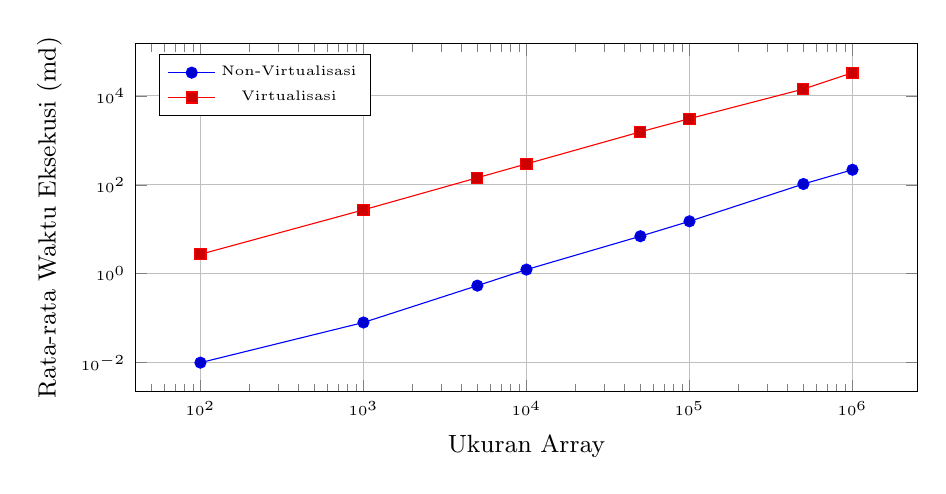
\begin{tikzpicture}
            \begin{axis}[
                    width=0.95\textwidth, height=6cm,
                    xlabel={Ukuran Array}, ylabel={Rata-rata Waktu Eksekusi (md)},
                    xmode=log, log basis x={10}, ymode=log, log basis y={10},
                    legend pos=north west, grid=major,
                    tick label style={font=\tiny}, label style={font=\small}, legend style={font=\tiny} ]
                \addplot coordinates { (100, 0.01) (1000, 0.08) (5000, 0.54) (10000, 1.24) (50000, 6.98) (100000, 15.12) (500000, 104.44) (1000000, 218.32) };
                \addlegendentry{Non-Virtualisasi};
                \addplot coordinates { (100, 2.74) (1000, 27.35) (5000, 144.44) (10000, 295.77) (50000, 1556.15) (100000, 3080.30) (500000, 14298.92) (1000000, 33292.91) };
                \addlegendentry{Virtualisasi};
            \end{axis}
        \end{tikzpicture}
        \caption{Perbandingan Waktu Eksekusi Quick Sort (Skala Log-Log).}
        \label{fig:quick_sort_performance_jurnal_ui_ana}
    \end{figure}

    \item \bo{Enkripsi AES:} Tabel \ref{tab:aes_performance_jurnal_ui_ana} menunjukkan bahwa total waktu untuk mengenkripsi 976MB data meningkat sekitar 396.7\% (1878.52 md menjadi 9330.73 md), dan waktu dekripsi meningkat sekitar 562.9\% (1304.75 md menjadi 8649.74 md). Akibatnya, \f{throughput} gabungan turun drastis dari 634.16 MB/s menjadi 108.78 MB/s (penurunan 82.8\%).
    % CATATAN: Anda perlu MENGISI DATA dari Tabel 5.6 dari skripsi Anda,
    % dan menyesuaikan label tabelnya menjadi unik untuk jurnal ini.
    \begin{table}[H]
        \centering
        \caption{Hasil Performa AES-256-CBC (Data 976MB)}
        \label{tab:aes_performance_jurnal_ui_ana}
        \fontsize{12}{12}\selectfont % Atur font size 10pt untuk tabel ini
        % SALIN KONTEN TABEL 5.6 DARI SKRIPSI ANDA KE SINI
        \begin{tabular}{@{}lrr@{}}
            \toprule
            \textbf{Metrik}              & \textbf{Non-Virtualisasi} & \textbf{Virtualisasi} \\
            \midrule
            Total Waktu Enkripsi (md)   & 1.878.52                 & 9.330.73             \\
            Total Waktu Dekripsi (md)   & 1.304.75                 & 8.649.74             \\
            % ... (Lanjutkan dengan data lainnya) ...
            Throughput Gabungan (MB/s)   & 634.16                   & 108.78               \\
            \bottomrule
        \end{tabular}
    \end{table}
\end{itemize}

\subsubsection{\f{Overhead} Ukuran Berkas}
Tabel \ref{tab:file_size_jurnal_ui_ana} menunjukkan peningkatan konsisten ukuran \f{executable} setelah virtualisasi. Untuk program konsol/benchmark yang lebih kecil, ukurannya meningkat lebih dari 15-18 kali lipat. Untuk aplikasi GUI yang lebih besar, peningkatan relatif lebih kecil namun tetap signifikan.
% CATATAN: Anda perlu MENGISI DATA dari Tabel 5.7 dari skripsi Anda,
% dan menyesuaikan label tabelnya menjadi unik untuk jurnal ini.
\begin{table}[H]
    \centering
    \caption{Perbandingan Ukuran Berkas Executable (KB)}
    \label{tab:file_size_jurnal_ui_ana}
    \fontsize{12}{12}\selectfont % Atur font size 10pt untuk tabel ini
    % SALIN KONTEN TABEL 5.7 DARI SKRIPSI ANDA KE SINI
    \begin{tabular}{@{}lrr@{}}
        \toprule
        \textbf{Program}  & \textbf{Non-Virtualisasi (KB)} & \textbf{Virtualisasi (KB)} \\
        \midrule
        quick\_sort       & 98                            & 1.537                     \\
        % ... (Lanjutkan dengan data lainnya) ...
        Lilith\_Client    & 84                            & 1.554                     \\
        \bottomrule
    \end{tabular}
\end{table}

\subsection{Diskusi}
Hasil eksperimen dengan jelas menunjukkan \textit{trade-off} inti dalam penggunaan virtualisasi kode VxLang.

\bo{Peningkatan Keamanan dan Penghindaran Deteksi:} VxLang memberikan penghalang substansial terhadap teknik rekayasa balik umum. Transformasi menjadi \f{bytecode} yang diinterpretasi menetralisir alat analisis statis standar seperti Ghidra \cite{Eilam2011, Ko2007} dan secara signifikan mempersulit analisis dinamis dengan alat seperti x64dbg, karena logika yang mendasarinya dieksekusi oleh VM buram \cite{Sikorski2012}. Hal ini sejalan dengan pemahaman mapan bahwa pengaburan berbasis VM secara fundamental mengubah struktur kode di luar kemampuan interpretasi \f{disassembler} standar \cite{Ore06, Salwan2018SymbolicDeobfuscation}. Lebih lanjut, analisis VirusTotal terhadap sepuluh sampel \f{malware}/PUA mengungkapkan dampak yang bernuansa: sementara VxLang dapat mengurangi deteksi berbasis \f{signature} untuk beberapa sampel, ia menyebabkan peningkatan deteksi untuk sampel lain, kemungkinan karena lapisan virtualisasi itu sendiri ditandai. Ini menyoroti interaksi kompleks antara pengaburan dan heuristik deteksi AV yang berkembang \cite{Ore06, Salwan2018SymbolicDeobfuscation, Rou13}.

\bo{Biaya Performa:} Manfaat keamanan dan penghindaran deteksi datang dengan harga performa yang mahal. \f{Overhead} interpretasi secara signifikan memperlambat kode tervirtualisasi, terutama untuk tugas-tugas komputasi intensif (\f{overhead} QuickSort ~15.000\% untuk 1 juta elemen; pengurangan \f{throughput} AES ~83\%), yang berpotensi membuat aplikasi yang tidak pandang bulu menjadi tidak praktis karena degradasi kecepatan yang parah.

\bo{Peningkatan Ukuran:} Peningkatan ukuran berkas yang cukup besar (misalnya, 15-18x untuk aplikasi kecil), terutama karena \textit{runtime} VM yang disematkan, merupakan faktor lain, khususnya relevan untuk aplikasi kecil atau kendala distribusi.

\bo{Implikasi Praktis:} VxLang tampak ampuh untuk melindungi kode yang sangat sensitif di mana keamanan dan potensi penghindaran deteksi adalah yang terpenting, dan dampak performa pada segmen spesifik tersebut dapat diterima (misalnya, anti-\f{tamper}, lisensi, IP inti). Kasus Lilith menunjukkan bahwa VxLang dapat melindungi logika kompleks tanpa merusaknya, \textbf{asalkan penempatan makro dilakukan dengan hati-hati dan iteratif untuk menghindari gangguan fungsionalitas, terutama pada bagian kode dengan alur kontrol kompleks atau operasi I/O}. Namun, biaya performa yang parah mengharuskan aplikasi strategis dan selektif, hanya menargetkan bagian kritis. Hasil VirusTotal juga menyiratkan bahwa meskipun profil deteksi diubah, penghindaran tidak dijamin. Pilihan antara autentikasi \f{hardcoded} dan berbasis \f{cloud} menunjukkan bahwa melindungi logika sisi klien yang menangani hasil validasi tetap krusial.
